\documentclass{standalone}

\usepackage{tikz}
\usetikzlibrary{calc}

\begin{document}

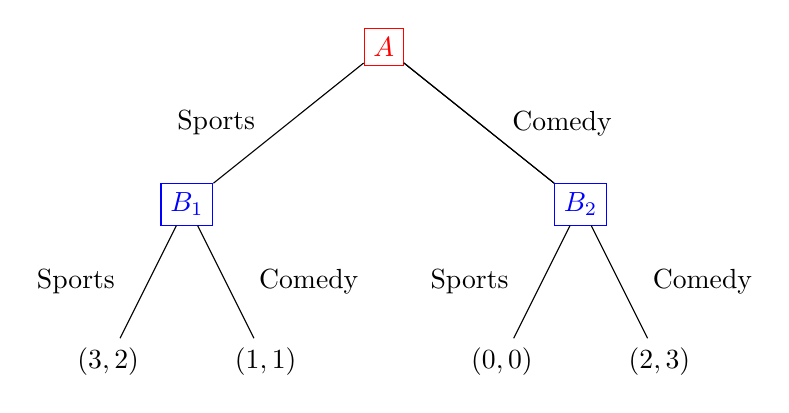
\begin{tikzpicture}
    \node [draw, color=red] (A) at (0, 0) {\(A\)};
        \node [draw, color=blue] (B1) at ($(A) + (-2.5, -2)$) {\(B_1\)};
            \node (SS) at ($(B1) + (-1, -2)$) {\((3, 2)\)};
            \node (SC) at ($(B1) + (1, -2)$) {\((1, 1)\)};
        \node [draw, color=blue] (B2) at ($(A) + (2.5, -2)$) {\(B_2\)};
            \node (CS) at ($(B2) + (-1, -2)$) {\((0, 0)\)};
            \node (CC) at ($(B2) + (1, -2)$) {\((2, 3)\)};

    \draw (A) -- node[left=3mm] {Sports} (B1);
    \draw (A) -- node[right=3mm] {Comedy} (B2);
        \draw (B1)  -- node[left=3mm] {Sports}  (SS);
        \draw (B1) -- node[right=3mm] {Comedy} (SC);
    \draw (A) -- (B2);
        \draw (B2)  -- node[left=3mm] {Sports}  (CS);
        \draw (B2) -- node[right=3mm] {Comedy} (CC);
\end{tikzpicture}

\end{document}
